% ==============================================================================
% فصل پنجم: پیکربندی ETMv4 و پیاده‌سازی Firmware
% ==============================================================================

\chapter{پیکربندی \lr{ETMv4} و پیاده‌سازی \lr{Firmware}}
\label{ch:firmware}

\section{مقدمه}
زیرسیستم ردیابی و عیب‌یابی \lr{CoreSight} در میکروکنترلرهای پیشرفته مبتنی بر معماری \lr{ARM Cortex-M7} (نظیر \lr{STM32H750})، مجموعه‌ای بسیار غنی از ماژول‌های مستقل سیلیکونی است که در فضای نگاشت‌شده حافظه (\lr{Memory-Mapped I/O}) قرار دارند. این ماژول‌ها پس از روشن شدن اولیه تراشه، به منظور جلوگیری از مصرف بیهوده توان و ممانعت از ایجاد تداخل‌های ناخواسته بر خطوط کلاک و پین‌های خروجی، در وضعیت کاملاً قفل‌شده و خاموش قرار دارند. راه‌اندازی این زیرسیستم بدون نقض شرط بنیادین «غیرتهاجمی بودن» (\lr{Non-Intrusiveness}) و بدون اعمال هرگونه اثر جانبی بر فرکانس و رفتار زمانی برنامه‌های کاربر، نیازمند مهندسی دقیق ترتیب پیکربندی ثبّات‌ها، مدیریت دامنه‌های توان و کلاک، و حل چالش‌های پنهان تطبیق معماری است.

در این فصل، ابتدا پروتکل فشرده‌سازی جریان دستورات در \lr{ETMv4} تبیین می‌گردد. سپس ساختار معماری زیرساخت دیباگ، دامنه‌های توان و توزیع کلاک در \lr{STM32H750} به همراه بلوک‌دیاگرام‌های مربوطه از راهنمای مرجع شرکت سازنده تشریح می‌شود. در ادامه، نگاشت حافظه و مراحل گام‌به‌گام پیکربندی ثبّاتی با تأکید بر ثبّات حیاتی \lr{TRCCONFIGR} بررسی شده و چالش بنیادین مغایرت راهنمای مرجع آی‌سی‌ها با استاندارد معماری \lr{ARM} تبیین می‌گردد. در بخش‌های بعدی، کالبدشکافی فایل‌های درایور مستقل \lr{\texttt{ETMv4.h}} و \lr{\texttt{ETMv4.c}} و روش به‌کارگیری محصول و تزریق به کدهای کاربری ارائه شده و در نهایت، ریشه‌یابی چالش بسته‌های همگام‌سازی (\lr{A-Sync}) و آسیب‌شناسی روش سوئیچینگ متناوب مستندسازی خواهد شد.

\section{پروتکل فشرده‌سازی جریان دستورات در \lr{ETMv4}}
\label{sec:etm_compression_protocol}
پردازنده \lr{Cortex-M7} در فرکانس‌های کاری چندصد مگاهرتزی، در هر ثانیه صدها میلیون دستورالعمل را اجرا می‌کند. ارسال بی‌درنگ و کامل آدرس ۳۲ بیتی هر دستورالعمل از طریق پایه‌های فیزیکی میکروکنترلر به پهنای باندی در مقیاس چند گیگابایت بر ثانیه نیاز دارد؛ در حالی که در عمل تنها یک گذرگاه موازی بسیار محدود (شامل یک خط کلاک و ۴ خط داده) در دسترس قرار دارد.

برای غلبه بر این محدودیت فیزیکی، استاندارد معماری \lr{ETMv4} شرکت \lr{ARM} از پروتکل فشرده‌سازی پیشرفته‌ای بر مبنای تفکیک رفتارهای خطی و غیرخطی پردازنده بهره می‌برد \cite{armetmv42017}:
\begin{enumerate}
    \item \textbf{ردیابی خطی و حذف آدرس‌ها:} تا زمانی که برنامه به صورت ترتیبی و بدون انشعاب دستورات متوالی حافظه را اجرا می‌کند، هیچ داده‌ای روی خط ردیابی ارسال نمی‌شود. دلیل این امر آن است که موتور دکودر نرم‌افزاری بر روی کامپیوتر میزبان، نسخه کامپایل‌شده باینری برنامه (\lr{.elf}) را در اختیار دارد؛ بنابراین با در دست داشتن آدرس اولیه، می‌تواند با دیس‌اسمبل کردن کد، نشانی دستورهای متوالی بعدی را خودش به صورت آفلاین محاسبه نماید.
    \item \textbf{بسته‌های انشعاب شرطی (\lr{Atom Packets}):} هنگامی که پردازنده به یک انشعاب شرطی (مانند دستورات \lr{\texttt{BEQ}}، \lr{\texttt{BNE}} یا عبارات \lr{if-else}) می‌رسد، ماژول \lr{ETM} تنها یک بیت وضعیت تولید می‌کند:
    \begin{itemize}
        \item کد \lr{E (Executed / Taken)}: نشان‌دهنده تحقق شرط و پرش به نشانی مقصد انشعاب.
        \item کد \lr{N (Not-Executed / Not-Taken)}: نشان‌دهنده عدم تحقق شرط و ادامه مسیر خطی برنامه.
    \end{itemize}
    سخت‌افزار \lr{ETM} جهت بیشینه‌سازی فشرده‌سازی، چندین اتم متوالی را در قالب یک بایت تجمیع کرده و به صورت بسته‌های تک‌بایتی به خروجی می‌فرستد.
    \item \textbf{بسته‌های همگام‌سازی (\lr{I\_SYNC} و \lr{A-Sync}):} به منظور بازیابی نقطه شروع اجرای برنامه یا هدایت دکودر در هنگام پرش‌های غیرمستقیم (نظیر فراخوانی توابع از طریق اشاره‌گرها، بازگشت از توابع یا ورود به توابع سرویس وقفه)، بسته‌های همگام‌سازی اجباری حاوی نشانی ۳۲ بیتی کامل ثبّات \lr{PC}، اطلاعات کانتکست و وضعیت کاری پردازنده ارسال می‌شوند.
    \item \textbf{برچسب‌های زمانی سخت‌افزاری (\lr{Timestamping}):} برای ارزیابی دقیق زمان سپری‌شده و همبسته‌سازی زمانی رویدادها، ماژول \lr{ETM} قادر است بسته‌های برچسب زمانی ۶۴ بیتی سراسری تولید کند.
    \item \textbf{شمارش چرخه‌های پردازنده (\lr{Cycle Counting - CCI}):} در کاربردهای تخمین بدترین زمان اجرا (\lr{WCET})، ثبت دقیق سیکل‌های سپری‌شده پردازنده بین دستورات حیاتی است. قابلیت \lr{CCI} با درج دلتای سیکل‌ها در جریان دستورات پایه، اندازه‌گیری چرخه-دقیق را بدون هیچ‌گونه سربار نرم‌افزاری فراهم می‌سازد.
\end{enumerate}

\section{معماری زیرساخت دیباگ، دامنه‌های توان و توزیع کلاک در \lr{STM32H750}}
\label{sec:debug_infra_architecture}
میکروکنترلر \lr{STM32H750} دارای زیرساخت عیب‌یابی و ردیابی بسیار پیچیده‌ای است که در راهنمای مرجع \lr{RM0433} شرکت \lr{STMicroelectronics} به تفصیل مستند شده است \cite{st2020stm32h7}. درک ساختار ارتباطی اجزای این زیرسیستم، تفکیک دامنه‌های توان و مدیریت کلاک‌های آنها پیش‌نیاز قطعی پیکربندی موفق \lr{Firmware} محسوب می‌شود.

\subsection{بلوک‌دیاگرام زیرساخت دیباگ و مسیر سیگنال‌های ردیابی}
شکل \ref{fig:debug_block_diagram} (برگرفته از شکل ۸۲۷ راهنمای مرجع \lr{RM0433})، معماری اتصالات داخلی اجزای دیباگ را نمایش می‌دهد.
\begin{figure}[H]
    \centering
    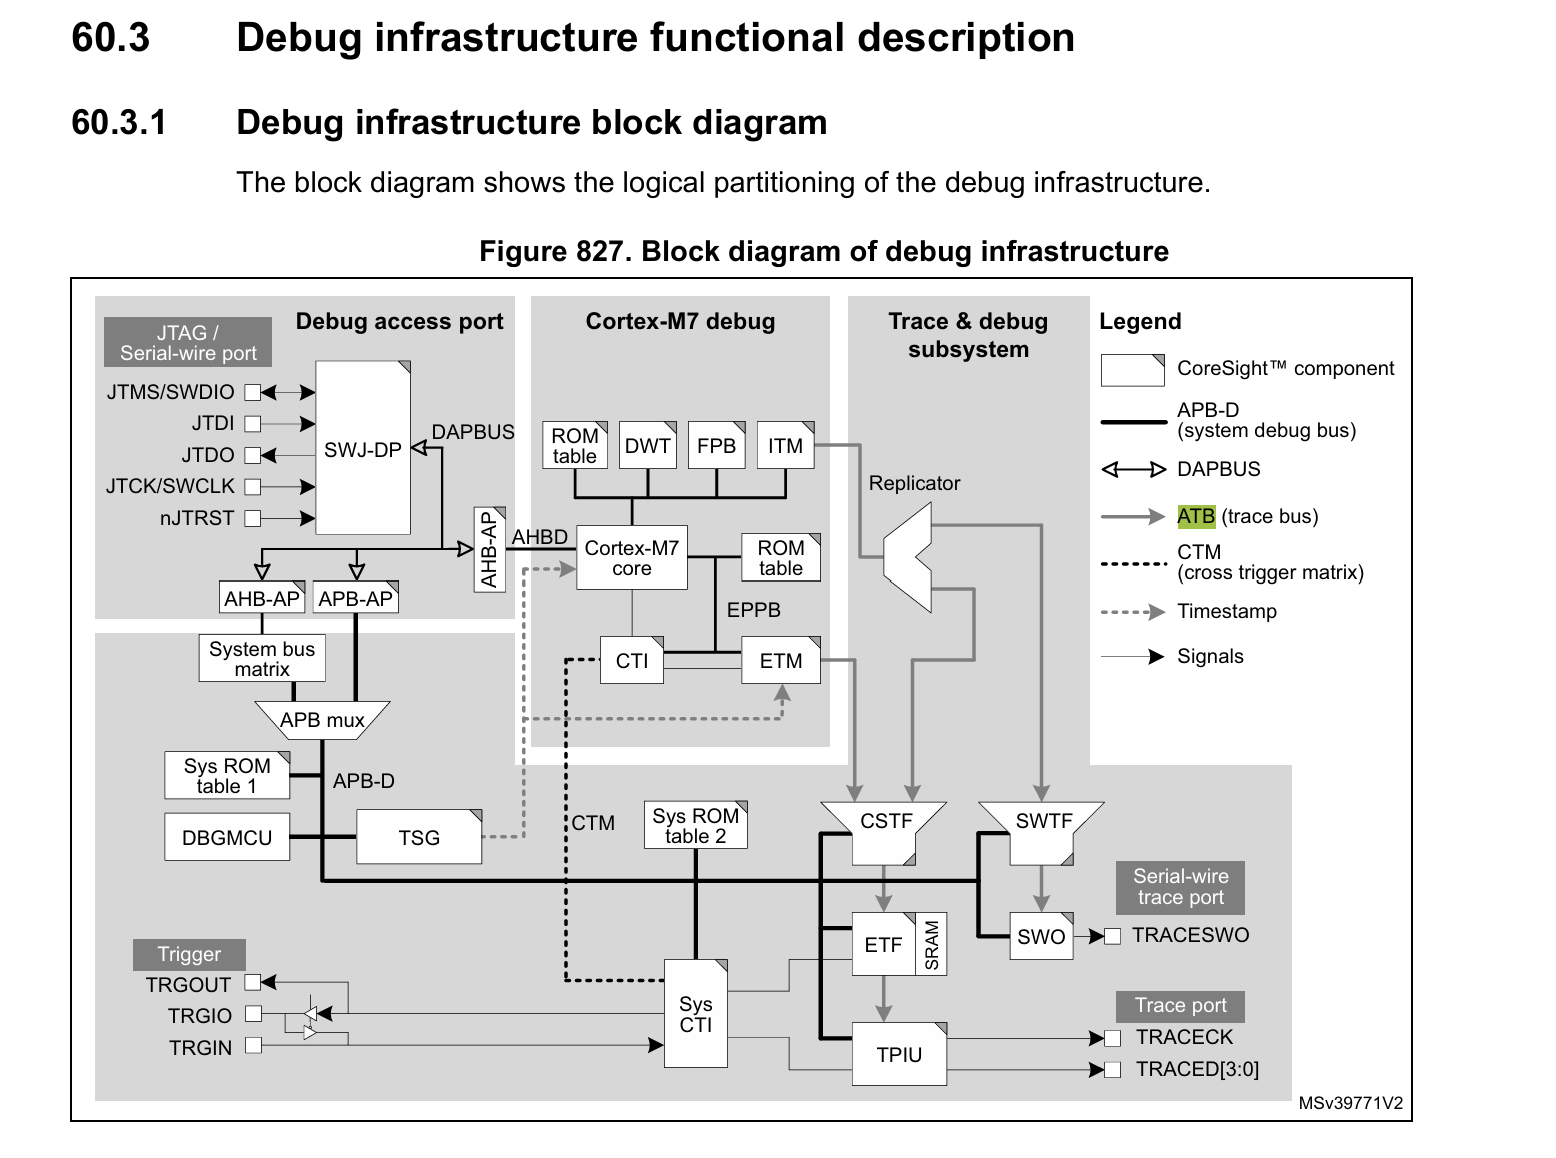
\includegraphics[width=0.88\textwidth]{figures/etm_pptx_image2.png}
    \caption{بلوک‌دیاگرام زیرساخت دیباگ و ردیابی در میکروکنترلر \lr{STM32H750} (شکل ۸۲۷  راهنمای مرجع \lr{RM0433})}
    \label{fig:debug_block_diagram}
\end{figure}

همان‌گونه که در شکل \ref{fig:debug_block_diagram} مشاهده می‌شود:
\begin{itemize}
    \item هسته پردازنده \lr{Cortex-M7} دربرگیرنده بلوک‌های \lr{ETMv4}، \lr{DWT} و \lr{ITM} است. ماژول \lr{ETMv4} پایش مستقیم گذرگاه دستورات پردازنده را بر عهده دارد.
    \item داده‌های ردیابی تولیدشده توسط \lr{ETM} و \lr{ITM} بر روی گذرگاه داخلی ۳۲ بیتی \lr{ATB (Advanced Trace Bus)} به سمت قیف ادغام ردیابی \lr{CSTF (CoreSight Trace Funnel)} هدایت می‌شوند.
    \item خروجی \lr{CSTF} وارد بافر سخت‌افزاری \lr{ETF (Embedded Trace FIFO)} می‌گردد. این بافر حافظه واسط، نوسانات شدید نرخ تولید بایت‌های \lr{Trace} در جهش‌های ناگهانی برنامه را مهار کرده و از سرریز داده‌ها جلوگیری می‌کند.
    \item در نهایت، جریان داده‌ها از خروجی \lr{ETF} وارد واحد فرمت‌بندی پورت ردیابی \lr{TPIU (Trace Port Interface Unit)} شده و این واحد، بایت‌ها را در قالب فریم‌های منظم سازمان‌دهی کرده و روی پورت موازی ۴ بیتی خارجی منتشر می‌سازد.
\end{itemize}

\subsection{دامنه‌های توان زیرساخت دیباگ (\lr{Power Domains})}
یکی از مهم‌ترین دلایل شکست تلاش‌های اولیه در راه‌اندازی ردیابی، عدم آگاهی از تفکیک دامنه‌های توان این ماژول‌ها در سیلیکون است. شکل \ref{fig:debug_power_domains} (برگرفته از شکل ۸۲۸ راهنمای مرجع \lr{RM0433}) دامنه‌های توان ماژول‌های دیباگ را تبیین می‌کند.
\begin{figure}[H]
    \centering
    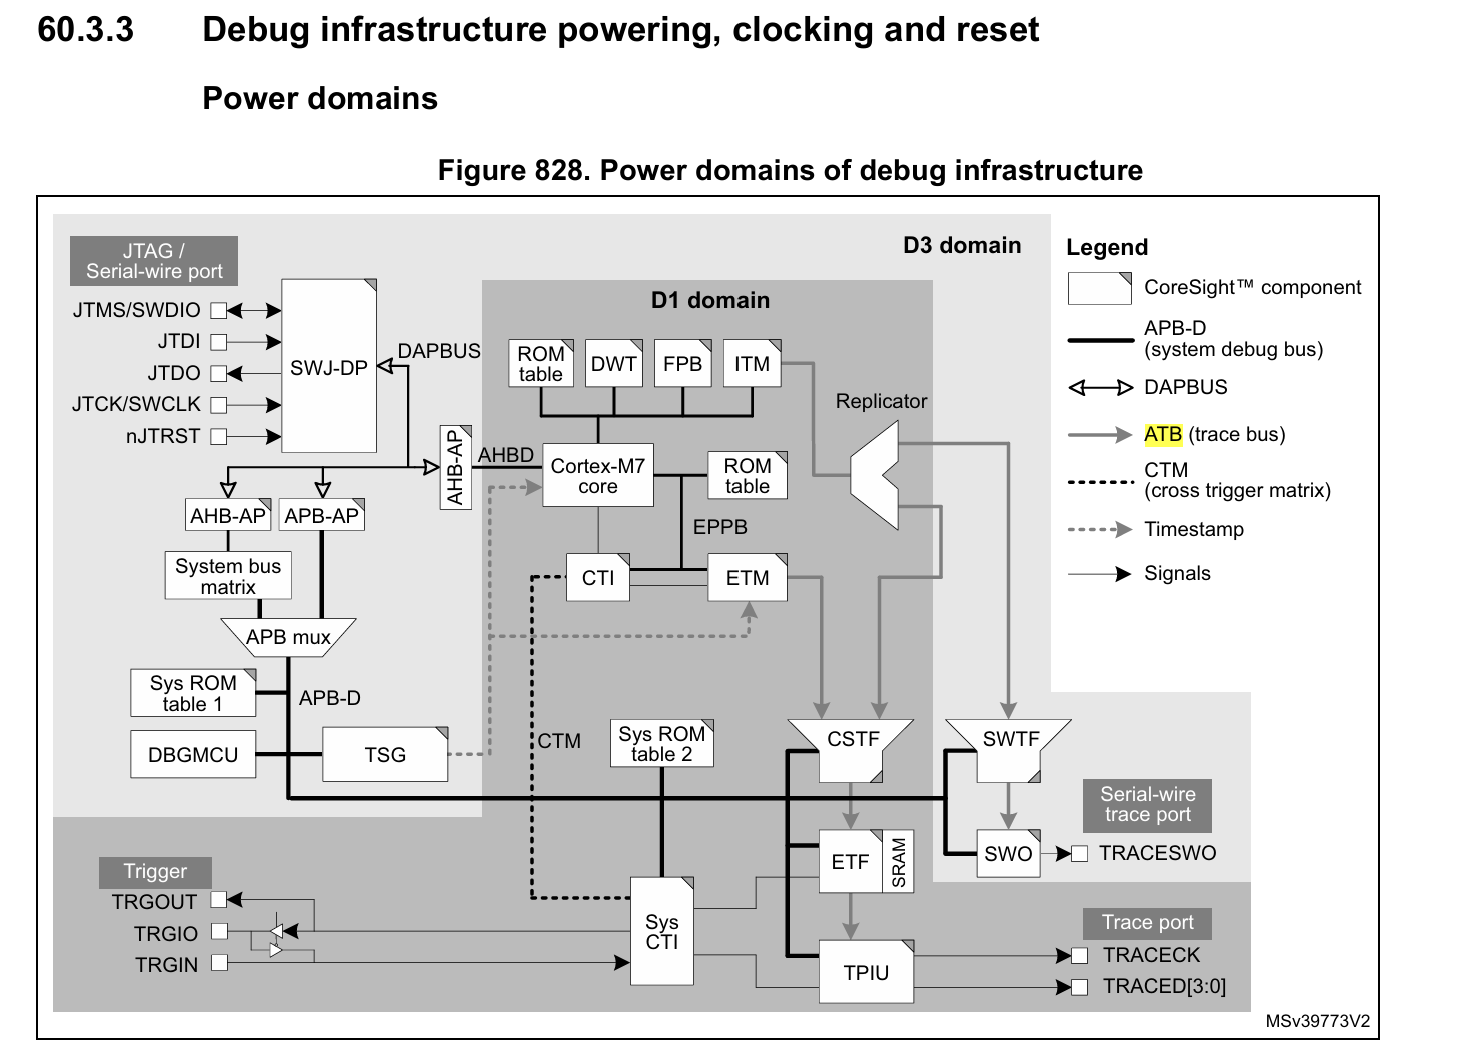
\includegraphics[width=0.85\textwidth]{figures/etm_pptx_image3.png}
    \caption{دامنه‌های توان زیرساخت دیباگ در میکروکنترلر \lr{STM32H750} (شکل ۸۲۸ راهنمای مرجع \lr{RM0433})}
    \label{fig:debug_power_domains}
\end{figure}

اجزای زیرسیستم ردیابی در دو دامنه توان متمایز قرار گرفته‌اند:
\begin{enumerate}
    \item \textbf{دامنه توان هسته (\lr{D1 Power Domain}):} هسته پردازنده \lr{Cortex-M7} و ماژول‌های محلی آن شامل \lr{ETMv4}، \lr{DWT} و \lr{ITM} در دامنه \lr{D1} قرار دارند. اگر هسته به مدهای کم‌توان (\lr{Sleep / Deep-Sleep}) وارد شود، برق این بخش قطع یا توان آن کاهش می‌یابد.
    \item \textbf{دامنه توان سیستم (\lr{D3 Power Domain}):} ماژول‌های زیرساختی شامل \lr{CSTF}، \lr{ETF}، \lr{TPIU}، \lr{DBGMCU} و درگاه \lr{SWO} در دامنه \lr{D3} قرار گرفته‌اند.
\end{enumerate}
بنابراین، \lr{Firmware} باید تضمین کند که هر دو دامنه \lr{D1} و \lr{D3} در وضعیت فعال کامل نگه داشته شوند و هیچ‌یک از اجزای مسیر ردیابی در حالت تعلیق توان قرار نگیرند.

\subsection{دامنه‌های کلاک زیرساخت دیباگ و اقدامات نرم‌افزاری}
شکل \ref{fig:debug_clock_domains} (برگرفته از شکل ۸۲۹ راهنمای مرجع \lr{RM0433}) مسیرهای توزیع کلاک را در زیرسیستم ردیابی نمایش می‌دهد.
\begin{figure}[H]
    \centering
    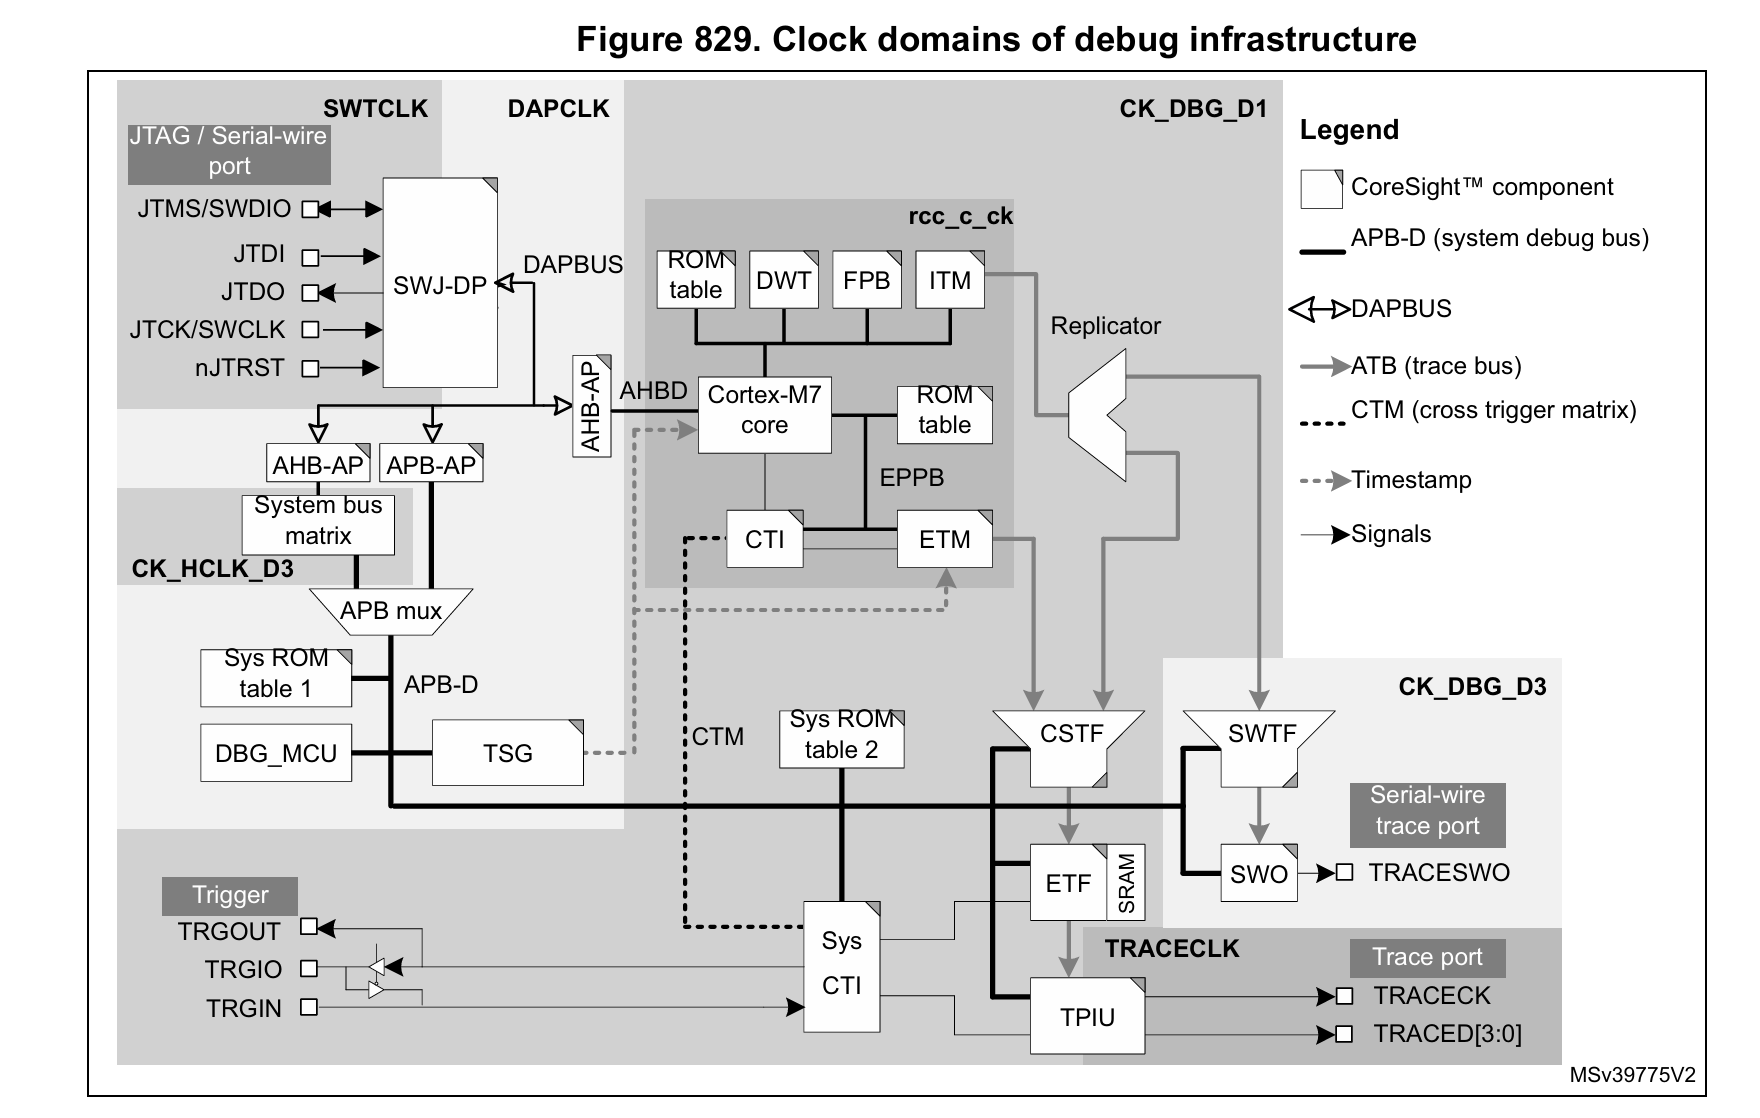
\includegraphics[width=0.88\textwidth]{figures/etm_pptx_image4.png}
    \caption{دامنه‌های کلاک زیرساخت دیباگ در میکروکنترلر \lr{STM32H750} (شکل ۸۲۹ راهنمای مرجع \lr{RM0433})}
    \label{fig:debug_clock_domains}
\end{figure}

در این ساختار، سه شبکه کلاک اساسی وجود دارد:
\begin{itemize}
    \item \textbf{کلاک هسته (\lr{CPU\_CLK}):} کلاک اصلی پردازنده که ماژول‌های \lr{ETMv4} و \lr{DWT} مستقیماً با آن کار می‌کنند. این موضوع تضمین می‌کند که ردیابی رویدادها دقیقاً با سرعت اجرای دستورات انجام می‌پذیرد.
    \item \textbf{کلاک خروجی ردیابی (\lr{TRACECLK / TRACECK}):} کلاکی که واحد \lr{TPIU} از آن برای کلاک کردن پین خروجی \lr{TRACECLK} (پایه \lr{PE2}) و تغییر وضعیت پایه‌های داده ردیابی استفاده می‌کند.
    \item \textbf{کلاک‌های گذرگاه دیباگ (\lr{DBG\_CKD1} و \lr{DBG\_CKD3}):} کلاک‌های فعال‌کننده دسترسی ثبّاتی به فضای \lr{CoreSight} در دامنه‌های \lr{D1} و \lr{D3}.
\end{itemize}

\textbf{اقدامات انجام‌شده در \lr{Firmware} جهت روشن کردن دامنه‌های کلاک و توان:}
برای فعال‌سازی کامل این مسیرها، کدهای راه‌انداز باید مراحل زیر را در ثبّات‌های سیستمی اعمال نمایند:
\begin{latin}
\begin{lstlisting}[language=C, caption={\rl{کد راه‌اندازی دامنه‌های توان و کلاک ردیابی در} \lr{DBGMCU} \rl{و} \lr{RCC}}]
/* 1. Enable GPIOE peripheral clock for trace output pins */
RCC->AHB4ENR |= RCC_AHB4ENR_GPIOEEN;

/* 2. Enable trace and debug monitor in CoreDebug */
CoreDebug->DEMCR |= CoreDebug_DEMCR_TRCENA_Msk; // Bit 24 (TRCENA = 1)

/* 3. Enable Trace clock, D1 debug clock, and D3 debug clock in DBGMCU */
DBGMCU->CR |= DBGMCU_CR_DBG_TRACECKEN | 
              DBGMCU_CR_DBG_CKD1EN     | 
              DBGMCU_CR_DBG_CKD3EN;
\end{lstlisting}
\end{latin}
بدون ست کردن همزمان بیت‌های فوق در ثبّات \lr{DBGMCU\_CR}، گذرگاه‌های \lr{ATB} و پورت \lr{TPIU} کلاک دریافت نکرده و کل سخت‌افزار ردیابی در وضعیت خاموش باقی خواهد ماند.

\section{نگاشت حافظه ثبّات‌های \lr{CoreSight} در \lr{STM32H750}}
در میکروکنترلر \lr{STM32H750}، هر یک از اجزای زیرسیستم ردیابی دارای یک بلوک آدرس ۴ کیلوبایتی در فضای دسترسی خصوصی پردازنده (\lr{Private Peripheral Bus - PPB}) یا گذرگاه \lr{AHB} هستند. جدول \ref{tab:coresight_registers} آدرس‌های پایه، دامنه‌های کاری و نقش هر مؤلفه را خلاصه نموده است \cite{st2020stm32h7}:

\begin{table}[H]
\centering
\caption{آدرس‌های پایه ماژول‌های \lr{CoreSight} در حافظه نگاشت‌شده \lr{STM32H750}}
\label{tab:coresight_registers}
\begin{tabularx}{\textwidth}{|l|c|c|X|}
\hline
\textbf{نام ماژول} & \textbf{آدرس پایه فیزیکی} & \textbf{دامنه} & \textbf{وظیفه معماری}\\
\hline
\lr{\texttt{ETMv4}} & \lr{\texttt{0xE0041000}} & \lr{PPB / D1} & موتور اصلی پایش دستورات، فشرده‌سازی شاخه‌ها و برچسب زمانی \\
\hline
\lr{\texttt{DWT}} & \lr{\texttt{0xE0001000}} & \lr{PPB / D1} & مقایسه‌گرهای آدرس، تریگرهای شروع/پایان و شمارنده چرخه \\
\hline
\lr{\texttt{DBGMCU}} & \lr{\texttt{0x5C001000}} & \lr{APB4 / D3} & کنترل کلاک‌های دیباگ، مدهای توان و فعال‌سازی \lr{Trace} \\
\hline
\lr{\texttt{TSG}} & \lr{\texttt{0x5C005000}} & \lr{AHB / D3} & تولیدکننده برچسب زمانی ۶۴ بیتی سراسری سیستم \\
\hline
\lr{\texttt{CSTF}} & \lr{\texttt{0x5C013000}} & \lr{AHB / D3} & قیف ادغام داده‌های \lr{Trace} و تخصیص شناسه جریان (\lr{Source ID}) \\
\hline
\lr{\texttt{ETF}} & \lr{\texttt{0x5C014000}} & \lr{AHB / D3} & بافر سخت‌افزاری \lr{FIFO} جهت جذب نوسانات ترافیک داده \\
\hline
\lr{\texttt{TPIU}} & \lr{\texttt{0x5C015000}} & \lr{AHB / D3} & فرمت‌بندی پورت موازی خارجی، تنظیم پهنای باند و فریم‌ها \\
\hline
\end{tabularx}
\end{table}

\section{مراحل گام‌به‌گام راه‌اندازی ثبّاتی}

\subsection{گام اول: آزادسازی قفل دسترسی نرم‌افزاری (\lr{Software Lock Removal})}
\label{subsec:software_lock}
مطابق با استاندارد معماری \lr{ARM CoreSight}، کلیه ثبّات‌های کنترلی و پیکربندی ماژول‌های ردیابی توسط مکانیزم قفل دسترسی نرم‌افزاری محافظت می‌شوند. تا پیش از باز شدن این قفل، هرگونه عملیات نوشتن در این ثبّات‌ها توسط سخت‌افزار نادیده گرفته شده و وضعیت مدار تغییر نمی‌کند.

برای باز کردن قفل هر ماژول، باید «کلید \lr{Lock Access Register}» (مقدار هگزادسیمال \lr{\texttt{0xC5ACCE55}}) در ثبّات \lr{LAR} (\lr{Lock Access Register}) در آفست \lr{\texttt{0xFB0}} ماژول مربوطه نوشته شود. پس از نوشتن این کلید، بیت ۱ در ثبّات وضعیت قفل (\lr{LSR - Lock Status Register}) در آفست \lr{\texttt{0xFB4}} پاک شده و مقدار صفر (نشان‌دهنده باز بودن قفل) را گزارش می‌دهد:

\begin{latin}
\begin{lstlisting}[language=C, caption={\rl{باز کردن قفل دسترسی نرم‌افزاری ماژول‌های} \lr{CoreSight} \rl{با استفاده از کلید} \lr{LAR}}]
#define CORESIGHT_UNLOCK_KEY  0xC5ACCE55UL
#define CORESIGHT_LAR_OFFSET  0xFB0UL
#define CORESIGHT_LSR_OFFSET  0xFB4UL

void CoreSight_Unlock_Component(uint32_t base_addr) {
    /* Write LAR unlock key to permit register write access */
    *((volatile uint32_t *)(base_addr + CORESIGHT_LAR_OFFSET)) = CORESIGHT_UNLOCK_KEY;
    __DSB(); // Ensure memory write completion
    
    /* Optional: poll LSR bit 1 until lock status indicates unlocked (0) */
    while (*((volatile uint32_t *)(base_addr + CORESIGHT_LSR_OFFSET)) & (1UL << 1));
}
\end{lstlisting}
\end{latin}

\subsection{گام دوم: پیکربندی پین‌های خروجی ردیابی (\lr{GPIOE Configuration})}
پورت موازی ردیابی در میکروکنترلر \lr{STM32H750} بر روی پین‌های درگاه \lr{GPIOE} نگاشت شده است. این پایه‌ها باید روی حالت عملگر دوم (\lr{Alternate Function 0 - AF0}) با بالاترین سرعت سوئیچینگ خروجی (\lr{Very High Speed}) تنظیم شوند:
\begin{itemize}
    \item پایه \lr{PE2}: سیگنال کلاک خروجی \lr{Trace} (\lr{TRACECLK})
    \item پایه‌های \lr{PE3} تا \lr{PE6}: خطوط ۴ بیتی داده ردیابی موازی (\lr{TRACED0} تا \lr{TRACED3})
\end{itemize}

\subsection{گام سوم: پیکربندی خط لوله ردیابی (\lr{CSTF}، \lr{ETF} و \lr{TPIU})}
مسیر عبور داده‌ها پس از تولید در هسته باید از میان ماژول‌های واسط هدایت گردد:
\begin{enumerate}
    \item \textbf{پیکربندی قیف ردیابی (\lr{CSTF}):} در ثبّات \lr{CTRL} ماژول \lr{CSTF}، پورت‌های متصل به هسته فعال شده و حداقل زمان نگهداری سوئیچینگ (\lr{Minimum Hold Time}) تنظیم می‌شود:
    \begin{latin}
    \begin{lstlisting}[language=C]
    CSTF->LAR  = CORESIGHT_UNLOCK_KEY;
    CSTF->CTRL = (0x3U << 8) | 0x1U; // Enable slave port with hold time = 3
    \end{lstlisting}
    \end{latin}
    \item \textbf{پیکربندی بافر سخت‌افزاری \lr{ETF}:} ماژول \lr{ETF} در مد \lr{Hardware FIFO} (مقدار \lr{\texttt{MODE = 0x02}}) پیکربندی می‌شود تا داده‌های ورودی از \lr{ATB} را مستقیماً در بافر رم داخلی قرار داده و با فعال بودن قالب‌بندی (\lr{\texttt{FFCR = 0x01}})، به سمت \lr{TPIU} پمپاژ نماید.
    \item \textbf{پیکربندی واحد پورت خارجی \lr{TPIU}:} اندازه پورت خروجی در ثبّات \lr{CURPSIZE} بر روی مقدار ۸ (معادل پورت ۴ بیتی) تنظیم گشته و ثبّات \lr{FFCR} با مقدار \lr{\texttt{0x00000002}} پر می‌شود که نشان‌دهنده فعال‌سازی حالت قالب‌بندی پیوسته (\lr{Continuous Formatting Mode}) است.
\end{enumerate}

\subsection[گام چهارم: پیکربندی موتور \lr{ETMv4} و تشریح دقیق ثبّات \lr{TRCCONFIGR}]{گام چهارم: پیکربندی موتور \lr{ETMv4}\\ و تشریح دقیق ثبّات \lr{TRCCONFIGR}}
\label{subsec:etm_config_register}
کلیدی‌ترین و سرنوشت‌سازترین ثبّات در کل فرآیند راه‌اندازی سخت‌افزار، ثبّات پیکربندی اصلی ردیابی \lr{ETM} موسوم به \lr{TRCCONFIGR} (یا \lr{M7\_ETM\_CONFIG}) در آفست \lr{\texttt{0x010}} است. این ثبّات به طور مستقیم قابلیت‌ها و ماهیت داده‌های خروجی ماژول \lr{ETM} را معین می‌سازد. شکل \ref{fig:rm0433_etm_config} ساختار بیت‌های این ثبّات را مطابق با راهنمای مرجع \lr{RM0433} نمایش می‌دهد.

\begin{figure}[H]
    \centering
    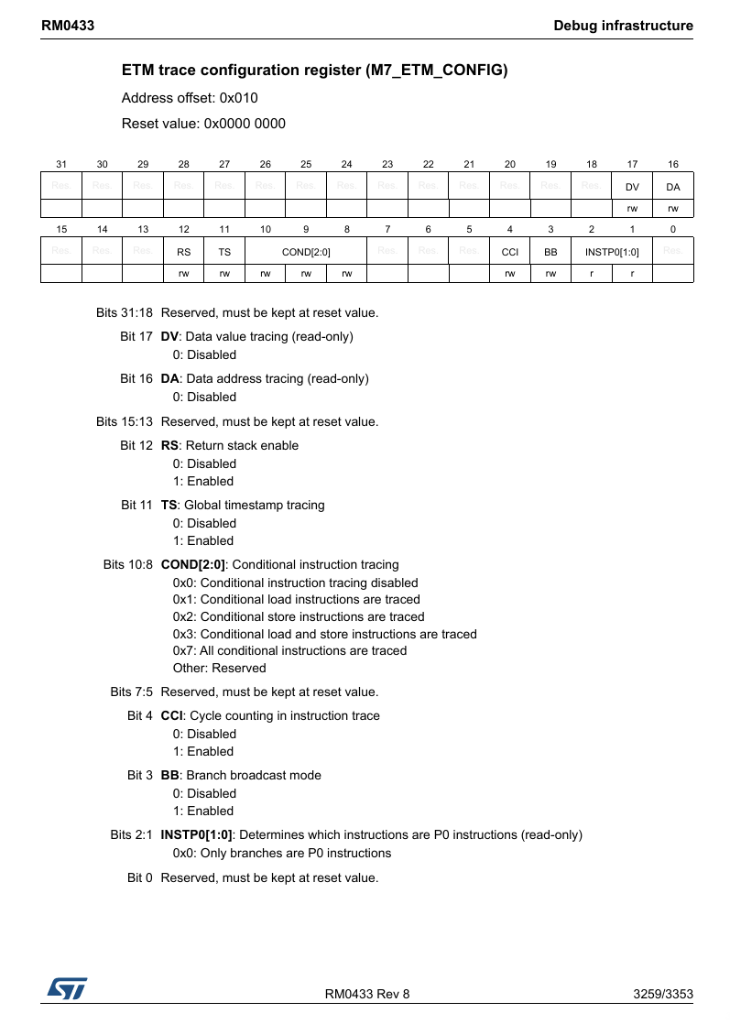
\includegraphics[width=0.88\textwidth]{figures/rm0433_etm_config_register.png}
    \caption{ساختار بیت‌های ثبّات پیکربندی ردیابی \lr{M7\_ETM\_CONFIG} برگرفته از راهنمای مرجع \lr{RM0433}}
    \label{fig:rm0433_etm_config}
\end{figure}

بررسی دقیق بیت‌های این ثبّات، مرز میان قابلیت‌های پیاده‌سازی‌شده در سیلیکون \lr{STM32H750} و مشخصات کلی استاندارد \lr{ARM} را آشکار می‌سازد:
\begin{itemize}
    \item \textbf{بیت ۱۷ (\lr{DV - Data Value Tracing}):} وضعیت فقط‌خواندنی (\lr{Read-Only}). در این پیاده‌سازی سخت‌افزاری، ردیابی مقادیر متغیرهای حافظه پشتیبانی نمی‌شود و همواره مقدار صفر دارد.
    \item \textbf{بیت ۱۶ (\lr{DA - Data Address Tracing}):} وضعیت فقط‌خواندنی (\lr{Read-Only}). ردیابی نشانی‌های داده پشتیبانی نمی‌شود و مقدار آن صفر است.
    \item \textbf{بیت ۱۲ (\lr{RS - Return Stack Enable}):} وضعیت خواندن/نوشتن (\lr{RW}). فعال کردن این بیت به ماژول \lr{ETM} اجازه می‌دهد پشته بازگشت توابع را در سخت‌افزار مدل‌سازی کند که منجر به کاهش فوق‌العاده بسته‌های انشعاب در هنگام بازگشت از زیربرنامه‌ها می‌شود.
    \item \textbf{بیت ۱۱ (\lr{TS - Global Timestamp Tracing}):} وضعیت خواندن/نوشتن (\lr{RW}). با فعال‌سازی این بیت، ماژول \lr{ETM} بسته‌های برچسب زمانی ۶۴ بیتی دریافت شده از مولد \lr{TSG} را در جریان داده‌ها منتشر می‌سازد که جهت اندازه‌گیری دقیق زمان دیوار ساعت (\lr{Wall-Clock Time}) ضروری است.
    \item \textbf{بیت‌های ۱۰ تا ۸ (\lr{COND[2:0] - Conditional Instruction Tracing}):} تعیین‌کننده نحوه پایش دستورات شرطی. مقدار \lr{\texttt{0b000}} پایش دستورات شرطی را غیرفعال کرده و مقدار \lr{\texttt{0b111}} تمامی دستورات شرطی را پایش می‌کند.
    \item \textbf{بیت ۴ (\lr{CCI - Cycle Counting in Instruction Trace}):} \textbf{حیاتی‌ترین بیت جهت سنجش \lr{WCET}}. فعال کردن این بیت سبب می‌شود ماژول \lr{ETM} دلتای تعداد چرخه‌های کلاک سپری‌شده هسته پردازنده را در جریان دستورات پایه (\lr{P0}) درج نماید. بدین ترتیب دکودر می‌تواند طول مدت اجرای هر بلوک را بر حسب چرخه‌های دقیق کلاک استخراج کند.
    \item \textbf{بیت ۳ (\lr{BB - Branch Broadcast Mode}):} در صورت فعال بودن، آدرس مقصد تمامی شاخه‌ها حتی شاخه‌های مستقیم را منتشر می‌سازد.
    \item \textbf{بیت‌های ۲ و ۱ (\lr{INSTP0[1:0]}):} وضعیت فقط‌خواندنی. مشخص‌کننده کلاس دستورات پایه (\lr{P0}) است که در این میکروکنترلر به شاخه‌ها محدود می‌باشد.
\end{itemize}

در پروژه حاضر، مقداردهی این ثبّات به صورت \lr{\texttt{ETM->CONFIG = (1U << 4) | (1U << 11);}} انجام گرفت که به طور همزمان قابلیت شمارش دقیق چرخه (\lr{CCI}) و برچسب زمانی سراسری (\lr{TS}) را برای سنجش چرخه‌ای \lr{WCET} فعال می‌سازد.

\subsection{چالش مغایرت راهنمای مرجع آی‌سی‌ها با مشخصات معماری \lr{ARM ETM}}
\label{subsec:spec_discrepancy}
یکی از مهم‌ترین یافته‌های تجربی و در عین حال اصلی‌ترین دلایل طولانی شدن فرآیند تحقیق و توسعه و پیکربندی اولیه سخت‌افزار در این پروژه، \textbf{شکاف عمیق و مغایرت ساختاری میان اسناد مرجع معماری شرکت \lr{ARM} و راهنمای مرجع سازندگان تراشه (\lr{STMicroelectronics})} بود.

در ابتدای فاز پیاده‌سازی، رویکرد متداول مهندسی ایجاب می‌کرد که از دستورالعمل رسمی شرکت \lr{ARM} در کتاب استاندارد معماری \lr{ETMv4} (\lr{ARM IHI 0064D}) استفاده شود. شکل \ref{fig:arm_spec_table} جدول معروف \lr{Table 4-15} این سند استاندارد را نشان می‌دهد که مراحل و مقادیر پیشنهادی \lr{ARM} را برای راه‌اندازی اولیه ردیابی دستورات مشخص کرده است \cite{armetmv42017}.

\begin{figure}[H]
    \centering
    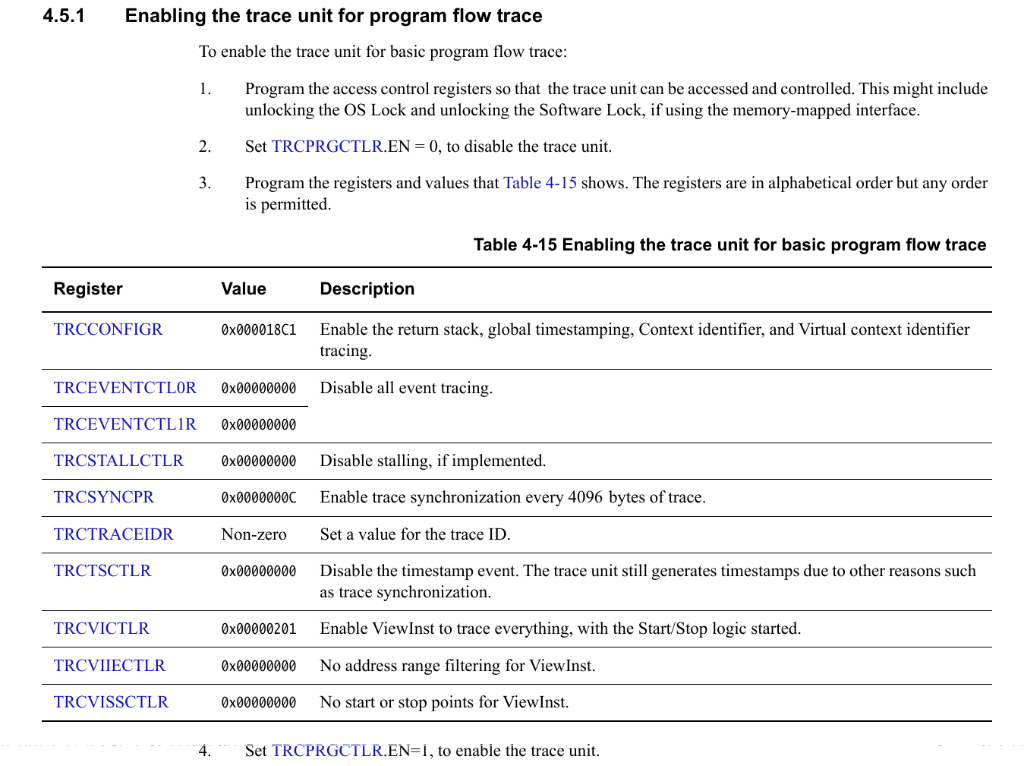
\includegraphics[width=0.88\textwidth]{figures/arm_etm_spec_enabling_table.png}
    \caption{دستورالعمل پیشنهادی فعال‌سازی ردیابی در استاندارد مرجع معماری \lr{ARM ETMv4} (جدول ۴-۱۵ سند \lr{ARM IHI 0064})}
    \label{fig:arm_spec_table}
\end{figure}

با این حال، پیاده‌سازی عینی و تلاش برای اجرای مستقیم مقادیر جدول \ref{fig:arm_spec_table} بر روی میکروکنترلر \lr{STM32H750} با شکست کامل مواجه شد. کالبدشکافی راهنمای مرجع \lr{RM0433} نشان داد که نمونه‌های ارائه‌شده در استاندارد \lr{ARM} بر روی پردازنده‌های واقعی قابل اجرای کورکورانه نیستند و هر ثبّات نیازمند تطبیق موشکافانه با جزئیات پیاده‌سازی سیلیکون است:
\begin{enumerate}
    \item \textbf{ثبّات‌های \lr{TRCVISSCTLR} و \lr{TRCVIIECTLR}:} در جدول ۴-۱۵ شرکت \lr{ARM}، صریحاً دستور داده شده که مقادیر این دو ثبّات صفر شوند تا فیلترینگ محدوده آدرس غیرفعال شود. اما در میکروکنترلر \lr{STM32H750}، ثبّات \lr{TRCVIIECTLR} اصلاً در سیلیکون پیاده‌سازی نشده و در فضای نگاشت حافظه وجود خارجی ندارد! همچنین ثبّات \lr{TRCVISSCTLR} بازطراحی شده و کنترل شروع/توقف به ثبّات‌های متفاوتی نظیر \lr{VIPCSSCTL} و \lr{VICTL} سپرده شده است. تلاش برای نوشتن در این آدرس‌ها موجب خطای دسترسی یا نادیده گرفته شدن فرمان می‌شود.
    \item \textbf{ثبّات دوره همگام‌سازی (\lr{TRCSYNCPR}):} در جدول پیشنهادی \lr{ARM}، نوشتن مقدار \lr{\texttt{0x0000000C}} (صدور همگام‌سازی هر ۴۰۹۶ بایت) توصیه شده است. اما در \lr{STM32H750}، این ثبّات از دید نرم‌افزار کاملاً \textbf{فقط‌خواندنی (\lr{Read-Only})} است و مقدار آن روی هگزادسیمال \lr{\texttt{0x0A}} ثابت نگه داشته شده است؛ بنابراین هرگونه تلاش نرم‌افزاری جهت نوشتن در این ثبّات بی‌اثر است.
    \item \textbf{مقداردهی ثبّات پیکربندی (\lr{TRCCONFIGR}):} شرکت \lr{ARM} در این جدول نوشتن مقدار \lr{\texttt{0x000018C1}} را پیشنهاد می‌دهد که بیت‌های ردیابی \lr{Context ID} و \lr{Virtual Context ID} را فعال می‌سازد. این بیت‌ها مختص پردازنده‌های رده کاربردی (\lr{Cortex-A}) با واحد مدیریت حافظه پیشرفته (\lr{MMU}) و هایپروایزر هستند. در پردازنده مایکروکنترلری \lr{Cortex-M7} این بیت‌ها یا رزرو هستند یا پیاده‌سازی نشده‌اند و نوشتن چنین مقداری وضعیت ثبّات را غیرقابل پیش‌بینی (\lr{UNPREDICTABLE}) می‌سازد.
\end{enumerate}

این مغایرت‌های بنیادین اثبات نمود که پیکربندی \lr{CoreSight} نیازمند مهندسی معکوس دقیق و اعتبارسنجی هر آفست حافظه بر اساس راهنمای مرجع اختصاصی تراشه (\lr{RM0433}) است و نمونه کدهای عمومی قابلیت اطمینان ندارند.

\section{تشریح فایل‌های راهکار نرم‌افزاری: پیاده‌سازی \lr{ETMv4.h} و \lr{ETMv4.c}}
\label{sec:firmware_implementation}
یکی از نکات حائز اهمیت در سطح معماری نرم‌افزار این است که \textbf{نه کتابخانه استاندارد هسته \lr{CMSIS} (\lr{\texttt{core\_cm7.h}}) و نه درایورهای شرکت سازنده (\lr{STM32Cube HAL})، هیچ‌گونه استراکت داده یا توابع رابطی برای ثبّات‌های \lr{ETMv4} در پردازنده \lr{Cortex-M7} فراهم نکرده‌اند!} شرکت \lr{ST} تنها ماژول‌های پایه‌ای \lr{DBGMCU} و درگاه تک‌سیمه \lr{SWO/ITM} را تعریف نموده است.

از این رو، کلیه ساختارهای داده نگاشت حافظه، ماسک‌های بیتی و توابع راه‌اندازی توسط نگارنده با مطالعه سطر به سطر اسناد \lr{RM0433 Rev 8} و \lr{ARM CoreSight v2.0} طراحی و پیاده‌سازی شد.

\subsection{ساختارهای داده در \lr{ETMv4.h}}
فایل هدر \lr{\texttt{ETMv4.h}} حاوی استراکت‌های کاملی از ماژول‌های سخت‌افزاری است:
\begin{itemize}
    \item \lr{\texttt{ETM\_TypeDef}}: ساختار کامل ثبّات‌های \lr{ETMv4} در آدرس \lr{\texttt{0xE0041000}} شامل ثبّات‌های کنترل برنامه‌ریزی (\lr{PRGCTL})، وضعیت (\lr{STAT})، پیکربندی (\lr{CONFIG})، شمارش چرخه (\lr{CCCTL})، شناسه ردیابی (\lr{TRACEID})، کنترل فیلترینگ (\lr{VICTL} و \lr{VIPCSSCTL}) و ثبّات‌های شناسایی سیلیکون (\lr{IDR0} تا \lr{IDR13}).
    \item \lr{\texttt{TPIU\_TypeDef}}: ساختار ثبّات‌های واحد اینترفیس پورت ردیابی در آدرس \lr{\texttt{0x5C015000}} شامل انتخاب اندازه پورت (\lr{CURPSIZE}) و کنترل قالب‌بندی و تخلیه (\lr{FFCR}).
    \item \lr{\texttt{CSTF\_TypeDef}}: ساختار قیف ردیابی در آدرس \lr{\texttt{0x5C013000}} جهت کنترل مالتی‌پبلکسر ورودی‌های \lr{ATB}.
    \item \lr{\texttt{ETF\_TypeDef}}: ساختار بافر \lr{FIFO} سخت‌افزاری در آدرس \lr{\texttt{0x5C014000}} جهت مدیریت جریان داده در مد \lr{Hardware FIFO}.
    \item \lr{\texttt{TSG\_TypeDef}}: ساختار مولد برچسب زمانی ۶۴ بیتی در آدرس \lr{\texttt{0x5C005000}}.
    \item \lr{\texttt{Trace\_Status\_t}}: ساختار جامع عیب‌یابی که با یک فراخوانی وضعیت تمامی ثبّات‌های مسیر ردیابی را در متغیر سراسری \lr{\texttt{g\_trace\_status}} کپی می‌کند تا در دیباگر قابل بازبینی باشد.
\end{itemize}

\subsection{توابع عملیاتی در \lr{ETMv4.c}}
پیاده‌سازی ارائه‌شده در \lr{\texttt{ETMv4.c}} شامل توابع کلیدی زیر است:
\begin{itemize}
    \item \lr{\texttt{Parallel\_Trace\_configure()}}: تابع اصلی راه‌اندازی که به ترتیب ماژول‌های پین خروجی، \lr{TPIU}، \lr{ETF}، \lr{CSTF}، \lr{TSG}، \lr{ETM} و \lr{DWT} را پیکربندی کرده و در نهایت ردیابی را فعال می‌سازد.
    \item \lr{\texttt{Disable\_ETM()}} و \lr{\texttt{Enable\_ETM()}}: وظیفه خاموش و روشن کردن ایمن هسته \lr{ETM}. تابع غیرفعال‌سازی پس از صفر کردن بیت \lr{PRGCTL.EN}، در یک حلقه منتظر ست شدن بیت‌های \lr{STAT.IDLE} و \lr{STAT.PMSTABLE} می‌ماند تا اطمینان حاصل شود خط لوله داخلی کاملاً تخلیه شده است.
    \item \lr{\texttt{DWT\_Configure()}}: مقایسه‌گرهای سخت‌افزاری شماره ۰ و ۱ ماژول \lr{DWT} را روی نشانی‌های شروع و پایان پنجره ردیابی تنظیم می‌کند.
    \item \lr{\texttt{StartPoint()}} و \lr{\texttt{StopPoint()}}: توابع نشانه‌گذار مرزهای اندازه‌گیری.
\end{itemize}

\textbf{راهکار ممانعت از بهینه‌سازی کامپایلر در توابع نشانه‌گذار:}
اگر توابع \lr{StartPoint} و \lr{StopPoint} صرفاً شامل دستورات توخالی یا مشابه‌ای مانند \lr{\texttt{nop}} باشند، بهینه‌ساز پیشرفته کامپایلر \lr{GCC} در سطوح بهینه‌سازی بالا (\lr{-Os} یا \lr{-O2}) به دلیل فعال بودن قابلیت \lr{-fipa-icf (Identical Code Folding)}، هر دو تابع را در یک نشانی یکسان در حافظه کد تجمیع می‌کند! در این صورت، نشانی تریگر شروع و پایان در \lr{DWT} برابر شده و هیچ ردیابی صورت نمی‌گیرد. برای شکستن این همسانی و ممانعت از ادغام توابع توسط کامپایلر، صفت \lr{\texttt{\_\_attribute\_\_((noinline))}} به همراه مقداردهی‌های متمایز به یک متغیر سراسری از جنس فرار (\lr{volatile}) درون توابع تزریق گردید:
\begin{latin}
\begin{lstlisting}[language=C, caption={\rl{پیاده‌سازی توابع نشانه‌گذار مرز پنجره با ممانعت از ادغام بهینه‌ساز}}]
volatile uint32_t g_gate_marker;

__attribute__((noinline)) void StartPoint(void){
    g_gate_marker = 0xA5A50001UL;
}

__attribute__((noinline)) void StopPoint(void){
    g_gate_marker = 0x5A5A0002UL;
}
\end{lstlisting}
\end{latin}

\section{روش به‌کارگیری محصول و تزریق به کدهای کاربری}
\label{sec:product_usage_workflow}
طراحی این سامانه با هدف سهولت بهره‌برداری در پروژه‌های صنعتی و دانشگاهی انجام شده است. برای استفاده از این سیستم تأمین داده ردیابی در پروژه‌های مختلف، فرآیند زیر طی می‌شود:
\begin{enumerate}
    \item افزودن فایل‌های درایور \lr{\texttt{ETMv4.h}} و \lr{\texttt{ETMv4.c}} به ساختار پروژه نرم‌افزاری میکروکنترلر.
    \item فراخوانی تابع راه‌انداز اصلی \lr{\texttt{Parallel\_Trace\_configure();}} در فاز مقداردهی اولیه سیستم (پیش از ورود به حلقه اصلی برنامه).
    \item احاطه کردن قطعه‌کد، تابع، یا حلقه مورد نظر جهت سنجش \lr{WCET} با دو فراخوانی ساده \lr{\texttt{StartPoint();}} و \lr{\texttt{StopPoint();}}.
\end{enumerate}

\subsection{تضمین عدم تداخل و حفظ رفتار غیرتهاجمی}
این روش به‌کارگیری، تضمین قطعی می‌دهد که \textbf{هیچ‌گونه تداخلی در رفتار زمانی، اولویت وقفه‌ها، یا منطق اجرایی سایر بخش‌های برنامه کاربر رخ نخواهد داد}. دلایل این قطعیت عبارتند از:
\begin{itemize}
    \item بلوک ردیابی \lr{ETM} به صورت مستقل و مستقیم با فرکانس اصلی پردازنده (\lr{CPU\_CLK}) کار می‌کند و هیچ سرباری بر خطوط لوله دستورات هسته تحمیل نمی‌نماید.
    \item تنظیمات زنجیره کلاک سیستم (\lr{PLL}ها)، مقسم‌های فرکانسی، کنترل‌کننده‌های وقفه (\lr{NVIC}) و پریفرال‌های کاربر بدون کمترین تغییر دست‌نخورده باقی می‌مانند.
    \item تنها تغییرات سخت‌افزاری اعمال‌شده، فعال‌سازی ماژول‌های زیرساخت دیباگ (\lr{CoreSight}) و تغییر پیکربندی پایه‌های اختصاصی ردیابی (\lr{PE2} تا \lr{PE6}) است که در کاربردهای عادی آزاد هستند.
\end{itemize}

\subsection{محدودیت نرخ‌های نمونه‌برداری سخت‌افزاری لاجیک آنالایزر}
نکته بسیار مهم در استفاده عملیاتی از این فرم‌ور، هماهنگی فرکانسی با ابزار گیرنده خارجی است. لاجیک آنالایزرهای دیجیتال (نظیر \lr{DSLogic U3Pro16}) از فرکانس‌های نمونه‌برداری گسسته و از پیش‌تعیین‌شده‌ای پشتیبانی می‌کنند. شکل \ref{fig:dslogic_sample_rates} منوی فرکانس‌های مجاز نمونه‌برداری در نرم‌افزار لاجیک آنالایزر مورد استفاده را نمایش می‌دهد.

\begin{figure}[H]
    \centering
    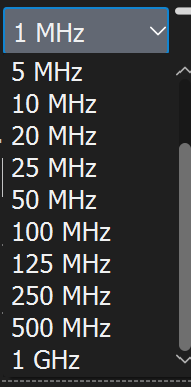
\includegraphics[width=0.35\textwidth]{figures/dslogic_sample_rates_menu.png}
    \caption{فرکانس‌های مجاز و گسسته نمونه‌برداری در نرم‌افزار لاجیک آنالایزر \lr{DSLogic}}
    \label{fig:dslogic_sample_rates}
\end{figure}

مطابق با شکل \ref{fig:dslogic_sample_rates}، نرخ‌های نمونه‌برداری دستگاه منحصراً به مقادیر ۱، ۵، ۱۰، ۲۰، ۲۵، ۵۰، ۱۰۰، ۱۲۵، ۲۵۰، ۵۰۰ مگاهرتز و ۱ گیگاهرتز محدود است. 

همان‌طور که در فصل چهارم اثبات شد، برای نمونه‌برداری پایدار و بدون خطای جیتر از لبه‌های کلاک پورت موازی، حداقل نسبت بیش‌نمونه‌برداری ۱۰ برابری ($10\times$) مورد نیاز است. کلاک پورت ردیابی (\lr{TRACECLK}) معمولاً نصف کلاک هسته پردازنده است ($f_{\mathrm{trace}} = f_{\mathrm{CPU}} / 2$). بنابراین:
\begin{itemize}
    \item اگر پردازنده در فرکانس ۲۰ مگاهرتز تنظیم شود، کلاک \lr{Trace} ۱۰ مگاهرتز بوده و با نرخ نمونه‌برداری ۱۰۰ مگاهرتز (۱۰ برابر) یا ۲۵۰ مگاهرتز (۲۵ برابر) لاجیک آنالایزر به طور کامل همخوانی دارد.
    \item اما اگر پردازنده در یک فرکانس کاری اختیاری غیرمنطبق (مثلاً ۴۸۰ مگاهرتز) تنظیم گردد، کلاک \lr{Trace} ۲۴۰ مگاهرتز خواهد شد که به نرخ نمونه‌برداری ۲.۴ گیگاهرتز نیاز دارد؛ نرخی که فراتر از سقف ۱ گیگاهرتزی لاجیک آنالایزر بوده و در منوی سخت‌افزار وجود ندارد.
\end{itemize}
بنابراین، در حال حاضر کاربر برای نمونه‌برداری معتبر سیگنال‌های \lr{Trace}، باید فرکانس کاری پردازنده را متناسب با نرخ‌های گسسته موجود در ابزار نمونه‌برداری انتخاب نماید.

\section[چالش بسته‌های همگام‌سازی (\lr{A-Sync}) و آسیب‌شناسی روش سوئیچینگ]{چالش بسته‌های همگام‌سازی (\lr{A-Sync})\\ و آسیب‌شناسی روش سوئیچینگ}
\label{sec:async_deep_dive}

\subsection[کشف ریشه خطای \lr{NO\_SYNC} و تصحیح وضعیت ثبّات \lr{TRCSYNCPR}]{کشف ریشه خطای \lr{NO\_SYNC}\\ و تصحیح وضعیت ثبّات \lr{TRCSYNCPR}}
\label{subsec:no_sync_issue}
در فازهای نخست پایش قطعه‌کدهای بسیار کوتاه (نظیر اجرای یک حلقه یا روتین وقفه با طول زمانی کمتر از ۵۰ میکروثانیه)، خطای عدم تطبیق در موتور دکودر \lr{OpenCSD} پدیدار می‌شد:
\begin{latin}
\begin{lstlisting}[language=bash]
OpenCSD: Trace un-synced - waiting for sync packet (NO_SYNC)
Error: Frame synchronization failed. 0 instructions reconstructed.
\end{lstlisting}
\end{latin}

کالبدشکافی جریان بایت‌ها ریشه این خطا را روشن ساخت:
\begin{itemize}
    \item دکودر نرم‌افزاری جهت تطبیق دادن بایت‌های فشرده اتم (\lr{E/N}) با باینری \lr{ELF}، لزوماً نیازمند دانستن «آدرس مبدأ مطلق» است که توسط بسته همگام‌سازی دستورالعمل (\lr{I\_SYNC / A-Sync}) حمل می‌شود.
    \item در معماری \lr{ETMv4}، ارسال بسته‌های \lr{I\_SYNC} بر عهده شمارنده داخلی است که دوره‌ای بودن آن به ثبّات \lr{TRCSYNCPR} منتهی می‌شود.
    \item \textbf{نکته حیاتی و تصحیح در گزارش:} در میکروکنترلر \lr{STM32H750}، ثبّات \lr{TRCSYNCPR} در سیلیکون به صورت کاملاً \textbf{فقط‌خواندنی (\lr{Read-Only})} پیاده‌سازی شده و مقدار آن به طور سخت‌افزاری بر روی مقدار هگزادسیمال \lr{\texttt{0x0A}} قفل است (معادل $2^{10} = 1024$ بایت). در نسخه‌های ابتدایی درایور، کدهایی جهت نوشتن مقادیر کوچکتری نظیر \lr{\texttt{0x08}} در این ثبّات وجود داشت؛ اما به دلیل ماهیت فقط‌خواندنی بودن، این عملیات توسط سخت‌افزار نادیده گرفته می‌شد.
    \item در قطعه‌کدهای کوتاه‌مدت، حجم کل داده‌های ردیابی تولیدشده تنها در حدود \textbf{۲۸ تا ۴۸ بایت} بود. از آنجا که حجم داده به سقف سخت‌افزاری ۱۰۲۴ بایت نمی‌رسید، سخت‌افزار هیچ بسته همگام‌سازی صادر نمی‌کرد و دکودر به دلیل فقدان نشانی اولیه قادر به رمزگشایی جریان نبود.
\end{itemize}

\subsection{روش ابداعی سوئیچینگ \lr{TRCPRGCTLR.EN} و آسیب‌شناسی آن}
\label{subsec:switching_drawbacks}
برای حل معضل بسته‌های همگام‌سازی، با اتکا به یک ویژگی معماری کشف‌شده در استاندارد \lr{ARM} مبنی بر این که:
\begin{quote}
\textit{«تغییر وضعیت بیت برنامه‌ریزی \lr{TRCPRGCTLR.EN} از صفر به یک، ماشین حالت \lr{ETM} را ریست کرده و سخت‌افزار را قانوناً ملزم می‌سازد تا در نخستین فریم خروجی، یک بسته همگام‌سازی اجباری اولیه (\lr{Initial I\_SYNC}) منتشر نماید.»}
\end{quote}
ایده خاموش و روشن کردن پویا و مقطعی ماژول \lr{ETM} در شروع هر پنجره آزمون پیاده‌سازی گردید. با این حال، ارزیابی‌های دقیق‌تر پرده از نقایص و خطرات این روش برداشت.

\textbf{مشکلات و آسیب‌شناسی روش خاموش و روشن کردن مکرر \lr{ETM}:}
\begin{enumerate}
    \item \textbf{از بین رفتن پیوستگی و یکپارچگی جریان ردیابی:} خاموش و روشن کردن پی‌درپی \lr{ETM} موجب شکستن پیوستگی زمانی داده‌ها می‌شود. در هر بار خاموش شدن، پایپ‌لاین فشرده‌سازی بازنشانی شده و تاریخچه ثبت شاخه‌ها پاک می‌گردد. در نتیجه، لاگ خروجی حاوی قطعات ناپیوسته و نامفهوم خواهد بود.
    \item \textbf{عدم تخلیه کامل بافر ردیابی (\lr{Buffer Drain Truncation}):} هنگامی که \lr{ETM} به صورت ناگهانی غیرفعال (\lr{Disable}) می‌شود، داده‌های ردیابی مربوط به آخرین دستورالعمل‌های اجراشده هنوز در بافرهای \lr{FIFO} داخلی ماژول و رم \lr{ETF} قرار دارند و فرصت انتقال کامل به پورت \lr{TPIU} را پیدا نکرده‌اند. در نتیجه، بخش انتهایی قطعه‌کد مورد سنجش دور ریخته شده یا با خطا مواجه می‌گردد.
\end{enumerate}

\textbf{راهکار مطمئن (\lr{Robust}) نهایی: \lr{Trace} ممتد در یک پنجره‌ و فیلترینگ نرم‌افزاری در دکودر:}
برای عبور بنیادین از این مشکلات، بهترین و قابل‌اعتمادترین رویکرد مهندسی آن است که:
\begin{itemize}
    \item ماژول \lr{ETM} در طول اجرای برنامه در یک پنجره زمانی متوالی، پیوسته روشن و فعال بماند تا هیچ بسته‌ای به دلیل قطع و وصل ناگهانی مفقود نگردد و یکپارچگی خط لوله فشرده‌سازی حفظ شود.
    \item در سمت کامپیوتر میزبان، اسکریپت دکودر پس از رمزگشایی کامل جریان بایت‌ها، در لاگ خروجی به جستجوی رخدادهای ورود به تابع \lr{StartPoint} و خروج از \lr{StopPoint} بپردازد.
\end{itemize}
گرچه این رویکرد به دلیل ثبت پیوسته دستورات حجم بایت‌های بیشتری تولید کرده و بار پردازشی دکودر را افزایش می‌دهد، اما داده‌هایی کاملاً یکپارچه، بدون مفقودی و فوق‌العاده مطمئن (\lr{Robust}) برای سنجش قطعی \lr{WCET} فراهم می‌سازد.

\section{جمع‌بندی فصل}
در این فصل پروتکل فشرده‌سازی داده‌ها در \lr{ETMv4}، معماری زیرساخت دیباگ در میکروکنترلر \lr{STM32H750} و دامنه‌های توان و کلاک آن تبیین شد. تشریح جامع ثبّات پیکربندی \lr{TRCCONFIGR}، ارائه شواهد مغایرت اسناد \lr{ARM} با راهنمای مرجع تراشه‌ها، معرفی فایل‌های درایور اختصاصی \lr{\texttt{ETMv4.h}} و \lr{\texttt{ETMv4.c}}، بررسی روش‌های به‌کارگیری و تزریق خودکار کد، و در نهایت ریشه‌یابی چالش بسته‌های \lr{A-Sync} و آسیب‌شناسی روش‌های سوئیچینگ \lr{ETM} مستند گردید. با تسلط بر این زیرساخت سخت‌افزاری و سیستم نرم‌افزاری روی تراشه، زمینه برای بررسی نحوه دریافت و رمزگشایی بایت‌ها در فصل ششم فراهم گردیده است.
